\documentclass[landscape,final]{baposter}

\usepackage[-1]{pagesel} % limit to one page

\usepackage{times}
\usepackage{calc}
\usepackage{graphicx}
\usepackage{amsmath}
\usepackage{amssymb}
\usepackage{relsize}
\usepackage{multirow}
\usepackage{bm}
\usepackage{epstopdf}
\usepackage{setspace}
\usepackage{graphicx}
\graphicspath{{images/}}
\usepackage{multicol}
\usepackage{mathtools,bm}
\usepackage{vwcol}

\usepackage{pgfbaselayers}
\pgfdeclarelayer{background}
\pgfdeclarelayer{foreground}
\pgfsetlayers{background,main,foreground}

\usepackage{helvet}
%\usepackage{bookman}
\usepackage{palatino}

\usepackage{wrapfig} % for text-wrapping figures



\newcommand{\captionfont}{\footnotesize}

\selectcolormodel{cmyk}

%\graphicspath{{images/}}

%\graphicspath{{figures/}}



%%%%%%%%%%%%%%%%%%%%%%%%%%%%%%%%%%%%%%%%%%%%%%%%%%%%%%%%%%%%%%%%%%%%%%%%%%%%%%%%
%%%% Some math symbols used in the text
%%%%%%%%%%%%%%%%%%%%%%%%%%%%%%%%%%%%%%%%%%%%%%%%%%%%%%%%%%%%%%%%%%%%%%%%%%%%%%%%

\newcommand{\CC}{\mathbb{C}}
\newcommand{\RR}{\mathbb{R}}
\newcommand{\LL}{\mathcal{L}}
\newcommand{\OO}{\mathcal{O}}

\newcommand{\veca}{\vec{a}}
\newcommand{\vecb}{\vec{b}}
\newcommand{\vecd}{\vec{d}}
\newcommand{\vece}{\vec{e}}
\newcommand{\vecf}{\vec{f}}
\newcommand{\vecn}{\vec{n}}
\newcommand{\vecp}{\vec{p}}
\newcommand{\vecr}{\vec{r}}
\newcommand{\vecu}{\vec{u}}
\newcommand{\vecv}{\vec{v}}
\newcommand{\vecw}{\vec{w}}
\newcommand{\vecx}{\vec{x}}
\newcommand{\vecy}{\vec{y}}
\newcommand{\vecz}{\vec{z}}


\renewcommand{\vec}[1]{\mathbf{#1}}

%%%%%%%%%%%%%%%%%%%%%%%%%%%%%%%%%%%%%%%%%%%%%%%%%%%%%%%%%%%%%%%%%%%%%%%%%%%%%%%%
% Multicol Settings
%%%%%%%%%%%%%%%%%%%%%%%%%%%%%%%%%%%%%%%%%%%%%%%%%%%%%%%%%%%%%%%%%%%%%%%%%%%%%%%%
\setlength{\columnsep}{0.7em}
\setlength{\columnseprule}{0mm}


%%%%%%%%%%%%%%%%%%%%%%%%%%%%%%%%%%%%%%%%%%%%%%%%%%%%%%%%%%%%%%%%%%%%%%%%%%%%%%%%
% Save space in lists. Use this after the opening of the list
%%%%%%%%%%%%%%%%%%%%%%%%%%%%%%%%%%%%%%%%%%%%%%%%%%%%%%%%%%%%%%%%%%%%%%%%%%%%%%%%
\newcommand{\compresslist}{%
\setlength{\itemsep}{1pt}%
\setlength{\parskip}{0pt}%
\setlength{\parsep}{0pt}%
}

\usepackage{enumitem}
\setlist[itemize,1]{leftmargin=\dimexpr 26pt-0.22in}

\DeclareMathSizes{10}{9}{7}{6}
\DeclareSymbolFont{extraup}{U}{zavm}{m}{n}
\DeclareMathSymbol{\vardiamond}{\mathalpha}{extraup}{87}

\newcommand{\headshotsize}{1.25in}




%%%%%%%%%%%%%%%%%%%%%%%%%%%%%%%%%%%%%%%%%%%%%%%%%%%%%%%%%%%%%%%%%%%%%%%%%%%%%%
%%% Begin of Document
%%%%%%%%%%%%%%%%%%%%%%%%%%%%%%%%%%%%%%%%%%%%%%%%%%%%%%%%%%%%%%%%%%%%%%%%%%%%%%

\begin{document}

%%%%%%%%%%%%%%%%%%%%%%%%%%%%%%%%%%%%%%%%%%%%%%%%%%%%%%%%%%%%%%%%%%%%%%%%%%%%%%
%%% Here starts the poster
%%%---------------------------------------------------------------------------
%%% Format it to your taste with the options
%%%%%%%%%%%%%%%%%%%%%%%%%%%%%%%%%%%%%%%%%%%%%%%%%%%%%%%%%%%%%%%%%%%%%%%%%%%%%%
\typeout{Poster Starts}
%\background{
%  \begin{tikzpicture}[remember picture,overlay]%
%    \draw (current page.north west)+(-2em,-0em) node[anchor=north west] {\hspace{-2em}\includegraphics[height=1.1\textheight]{silhouettes_background}};
%  \end{tikzpicture}%
%}

\definecolor{cuGold}{cmyk}{0, .10, .48, .22}
\definecolor{cuBlack}{cmyk}{0, 0, 0, 1.00}
\definecolor{cuDarkGray}{cmyk}{.38, .28, .21, .63}
\definecolor{cuLightGray}{cmyk}{.16, .11, .11, .29}

\begin{poster}{
	% Show grid to help with alignment
	grid=no,
	columns=4,
	% Column spacing
	colspacing=1em,
	% Color style
	bgColorOne=cuBlack,
	bgColorTwo=cuBlack,
	borderColor=cuGold,
	headerColorOne=cuDarkGray,
	headerColorTwo=black,
	headerFontColor=white,
	%  headerFontColor=black,
	%  boxColorOne=lightestblue,
	%  boxColorTwo=lightestblue,
	boxColorOne=white,
	boxColorTwo=white,
	% Format of textbox
	%textborder=roundedleft,
	textborder=rounded,
	% Format of text header
	eyecatcher=yes,
	headerborder=closed,
	headerheight=0.11\textheight,
	%  headershape=rectangle,
	headershape=rounded,
	headershade=plain,
	headerfont=\Large\textsf, %Sans Serif
	boxshade=plain,
	%  background=shade-tb,
	background=plain,
	linewidth=2pt
}
% University logo 
{{\begin{minipage}{4.5in}

\includegraphics[height=10em]{cu_logo}
%%%%%%%%%%%%%%%%%%%%%%%%%%%%%%%%%%%%%%%%%%%%%%%%%%%%%%%%%%%%%%%%%%%%%%%%%%%%%%%%%%%%%%%%%%
\end{minipage}}} % No eye catcher for this poster. If an eye catcher is present, the title is centered between eye-catcher and logo.
% Title
{
	\bf \huge
	\color{cuGold}
	%Input-Response Relations for Traveling Waves\\in Neural Fields with Synaptic Depression
	Stimuli shift the position of traveling waves \\in neural fields with synaptic depression
	\vspace{1mm}
}
% Authors
{\sc\large 
\color{cuGold}
	Sage B. Shaw and Zachary P. Kilpatrick\\ University of Colorado Boulder
}
% Headshots
{{\begin{minipage}{4.5in}
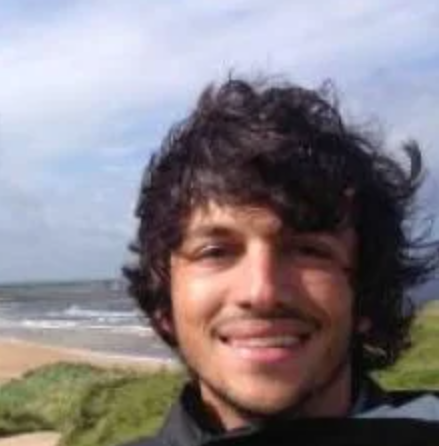
\includegraphics[height=\headshotsize, trim={5.1cm, 6cm, 2cm, 0cm}, clip=true]{headshot_zack}
\hspace{.5cm}

\includegraphics[height=\headshotsize, trim={3cm, 0cm, 3cm, 0cm}, clip=true]{headshot_sage}
\hspace{.5cm}
\includegraphics[height=\headshotsize]{NSF_logo.eps}
%
\includegraphics[height=\headshotsize]{QR.eps}
\end{minipage}}}

%\tikzstyle{light shaded}=[top color=baposterBGtwo!30!white,bottom color=baposterBGone!30!white,shading=axis,shading angle=30]

  % Width of left inset image
     \newlength{\leftimgwidth}
     \setlength{\leftimgwidth}{0.78em+8.0em}

%%%%%%%%%%%%%%%%%%%%%%%%%%%%%%%%%%%%%%%%%%%%%%%%%%%%%%%%%%%%%%%%%%%%%%%%%%%%%%
%%% Now define the boxes that make up the poster
%%%---------------------------------------------------------------------------
%%% Each box has a name and can be placed absolutely or relatively.
%%% The only inconvenience is that you can only specify a relative position 
%%% towards an already declared box. So if you have a box attached to the 
%%% bottom, one to the top and a third one which should be in between, you 
%%% have to specify the top and bottom boxes before you specify the middle 
%%% box.
%%%%%%%%%%%%%%%%%%%%%%%%%%%%%%%%%%%%%%%%%%%%%%%%%%%%%%%%%%%%%%%%%%%%%%%%%%%%%%
    %
%    % A coloured circle useful as a bullet with an adjustably strong filling
%    \newcommand{\colouredcircle}[1]{%
%      \tikz{\useasboundingbox (-0.2em,-0.32em) rectangle(0.2em,0.32em); \draw[draw=black,fill=baposterBGone!80!black!#1!white,line width=0.03em] (0,0) circle(0.18em);}}

%%%%%%%%%%%%%%%%%%%%%%%%%%%%%%%%%%%%%%%%%%%%%%%%%%%%%%%%%%%%%%%%%%%%%%%%%%%%%%
\headerbox{Summary}{name=summary,column=0,row=0}{
	 \textbf{Scientific Question:} \textbf{How do brains encode and predict motion?}
	 \begin{itemize}
		 \item The firing-rate of populations of neurons is sufficient to explain dynamics of large-scale neural networks.
		 \item We can approximate large discrete networks using integro-differential equations called \textit{neural field models}.
		 \item Synaptic depression allows for biologically realistic traveling pulses in neural field models.
		 \item External stimuli can adjust the position of traveling pulses.
	 \end{itemize}
	 \vspace{.05cm}
}

\headerbox{Background: Synaptic Depression}{name=background, column=0, below=summary}
{
	\begin{itemize}
	\item When a pre-synaptic neuron fires, it releases neurotransimiters into the synaptic cleft separating it from the post-synaptic neuron.
	\item When neurons fire repeatedly, they will deplete their store of neurotransmiters faster than they replenish them.
	\item This results in reduced stimulation of the post-synaptic neuron and a reduced firing-rate. We call this \textbf{synaptic depression}.
	\end{itemize}	
	\vspace{-.7cm}
	\begin{center}
	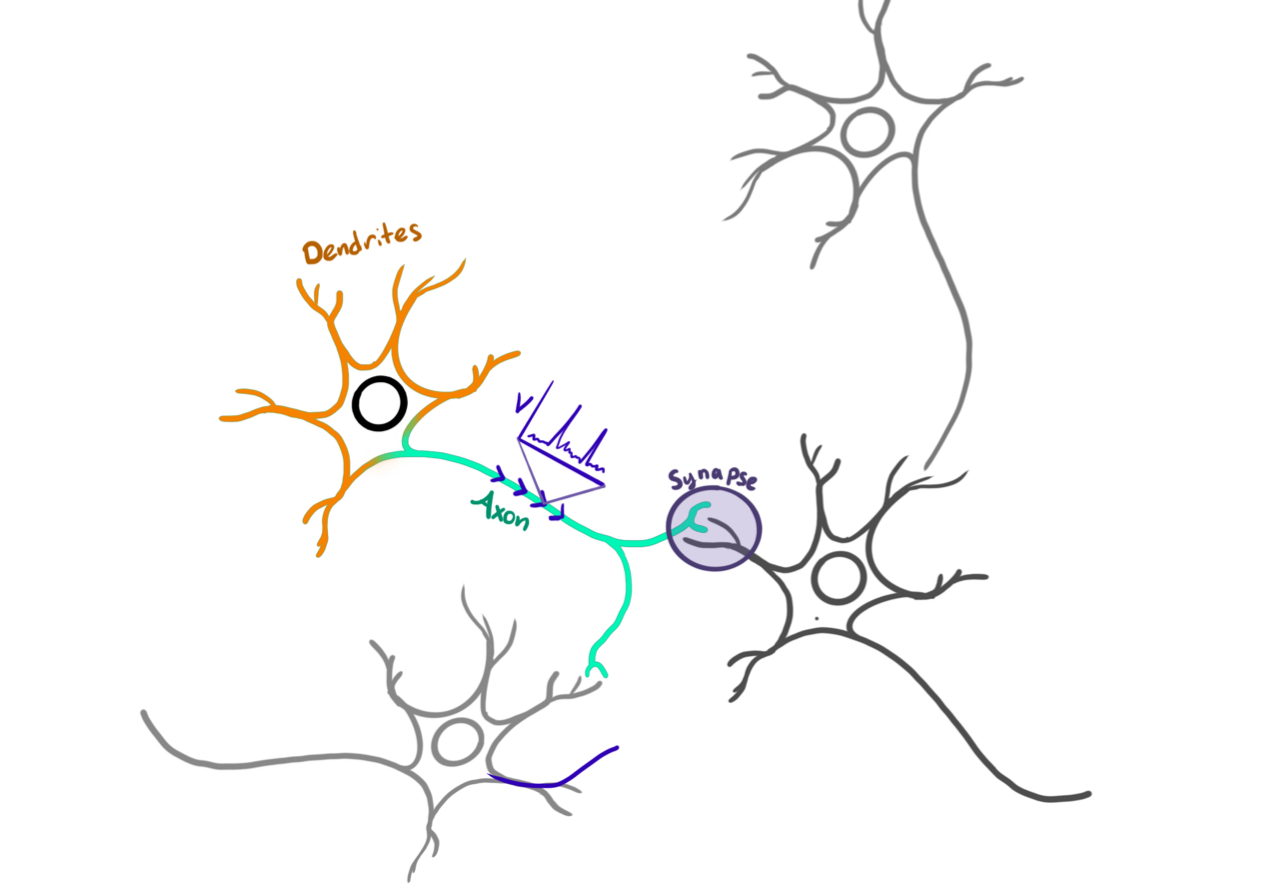
\includegraphics[width=.9\linewidth, trim={6cm, 6cm, 0cm, 10cm}, clip=true]{synapse} \\
	Image courtesy of Heather Cihak.
	\end{center}
}

%%%%%%%%%%%%%%%%%%%%%%%%%%%%%%%%%%%%%%%%%%%%%%%%%%%%%%%%%%%%%%%%%%%%%%%%%%%%%%
\headerbox{One-Dimensional Neural-Field Model}{name=model,column=0, below=background, above=bottom}
{
	\begin{align*}
		\tau_u \frac{\partial}{\partial t} u(x, t) &= \underbrace{-u(x,t)}_{\text{decay}} + \underbrace{\int_\RR w(|x-y|) \ q(y, t) f\big[u(y, t)\big] \ dy}_{\text{non-linear spatial operator}} + \underbrace{\varepsilon I_u(x, t)}_{\text{stimulus}}\\
		\tau_q \frac{\partial}{\partial t} q(x, t) &= \underbrace{1 - q(x,t)}_{\text{replenishment}} - \underbrace{\beta q(x,t) f\big[u(x, t)\big]}_{\text{depletion}} + \underbrace{\varepsilon I_q(x,t)}_{\text{stimulus}}
	\end{align*}
	\vspace{-.5cm}
	\begin{align*}
		w(|x-y|) &= \tfrac{1}{2}e^{-|x-y|} & \gamma &= \frac{1}{1+\beta} \\
		f(\cdot) &= H(\cdot - \theta) & A(t) &= \{x \in \RR \mid u(x,t) \ge \theta \}
	\end{align*}
	\begin{itemize}
		\item $u(x,t)$ -- neural activity (normalized firing-rate)
		\item $q(x,t)$ -- synaptic efficacy ($q<1$ represents synaptic depression)
		\item $\tau_u$ -- time-scale of neural activity
		\item $\tau_q$ -- time-scale of synaptic repleneshment
		\item $\beta$ -- time-scale (relative to $\tau_q$) of synaptic depletion
		\item $\gamma$ -- effective synaptic time-scale (relative to $\tau_q$)
		\item $w$ -- a weight kernel that encodes the network connectivity
		\item $f$ -- a non-linear firing-rate function
		\item $\theta$ -- the firing-rate threshold
		\item $A(t)$ (active region) -- the subset of domain in which neural activity is sufficient to simtulate other areas of the network
		\item $\varepsilon I_u, \varepsilon I_q$ -- small external stimulii
	\end{itemize}
	
}
%%%%%%%%%%%%%%%%%%%%%%%%%%%%%%%%%%%%%%%%%%%%%%%%%%%%%%%%%%%%%%%%%%%%%%%%%%%%%%
\headerbox{Traveling Wave Solutions}{name=solutions,column=1,row=0,height=1.0}
{
	\begin{itemize}
		\item Convert to characteristic coordinates: $\xi = x - c t$
		\item Traveling wave solutions $u(x,t) = U(\xi), \ q(x,t) = Q(\xi)$ satisfy the linear system
			\begin{align*}
				-c\tau_u \frac{d}{d \xi} U(\xi) &= -U(\xi) + \int_A w(|\xi - y|) Q(y) \ d\xi' \\
				-c \tau_q \frac{d}{d \xi} Q(\xi) &= 1 - Q(\xi) - \beta Q(\xi) I_A(\xi)
			\end{align*}
		\item This gives a consistency equation for the speed $c$ (and pulse width).
	\end{itemize}
	\begin{center}
		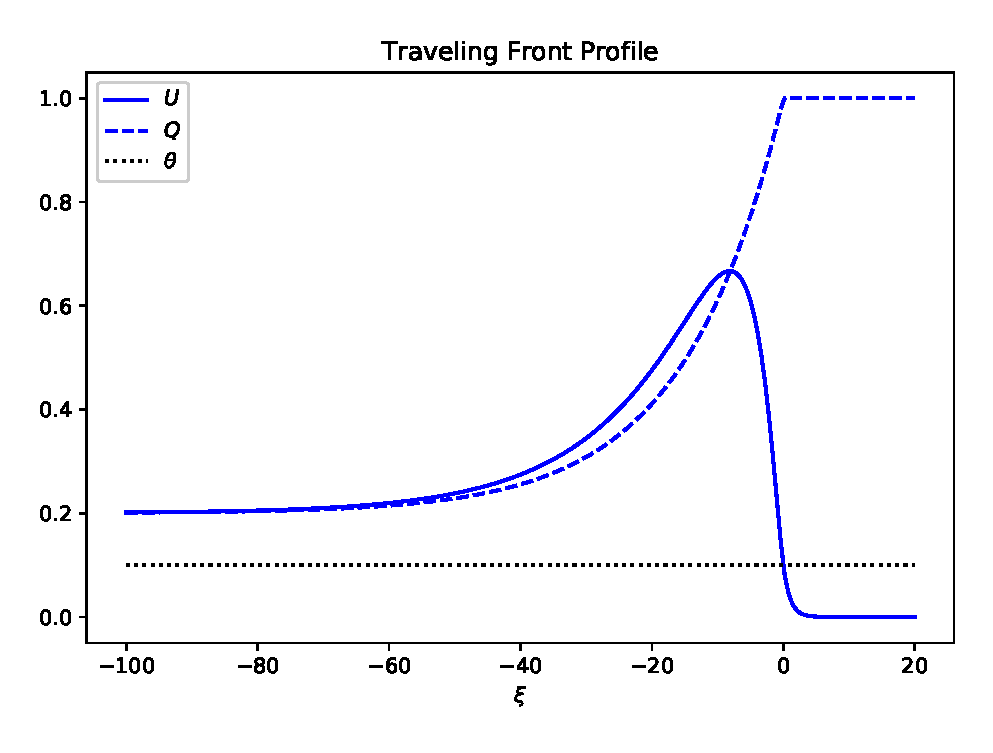
\includegraphics[width=.9\linewidth, trim={0cm, .2cm, 0cm, 0cm}, clip=true]{front_profile}
		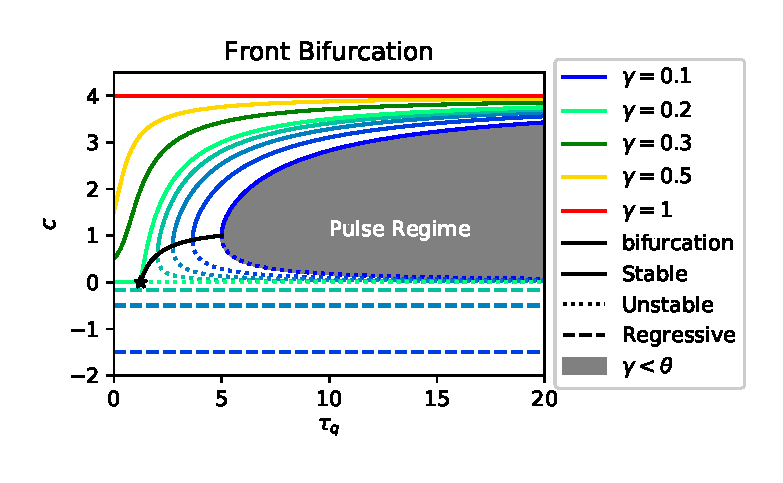
\includegraphics[width=.9\linewidth, trim={0cm, .2cm, 0cm, 0cm}, clip=true]{front_bifurcation}
		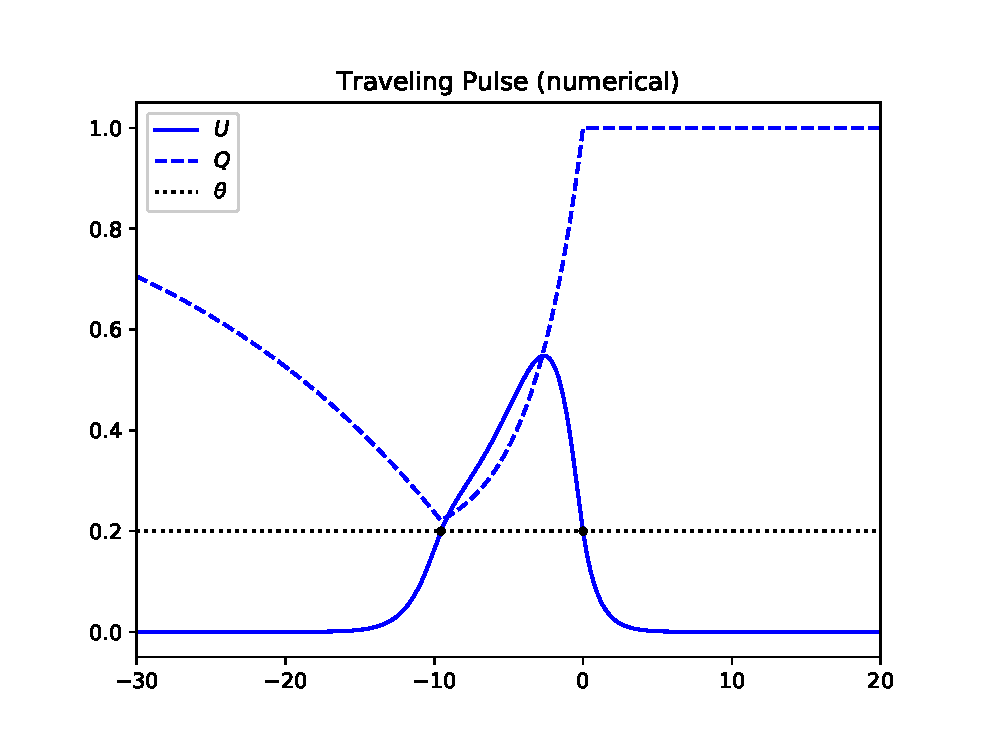
\includegraphics[width=.9\linewidth, trim={0cm, .2cm, 0cm, 0cm}, clip=true]{pulse_profile}
		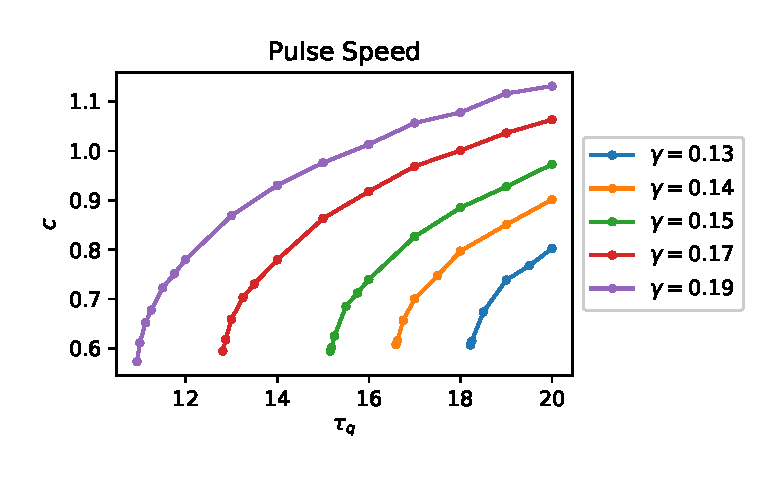
\includegraphics[width=.9\linewidth, trim={0cm, 1cm, 0cm, .2cm}, clip=true]{pulse_speed}
	\end{center}
}

%\headerbox{Traveling Pulse Solutions}{name=solutions2,column=1,below=solutions,above=bottom}
%{
%	\begin{center}
%		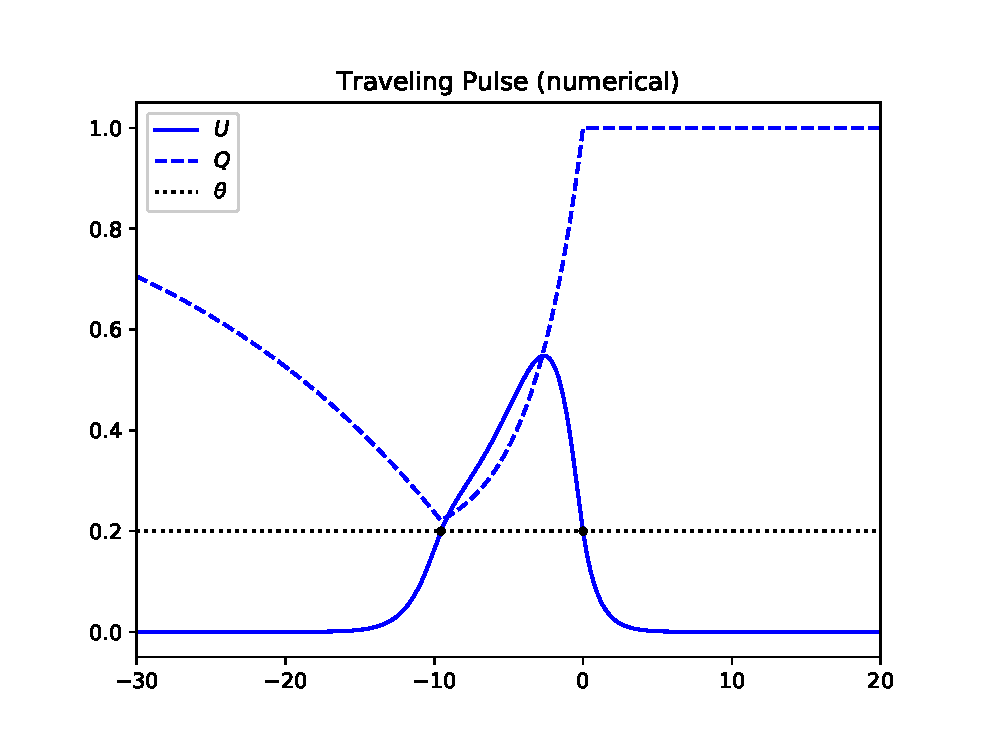
\includegraphics[width=.9\linewidth]{pulse_profile}
%		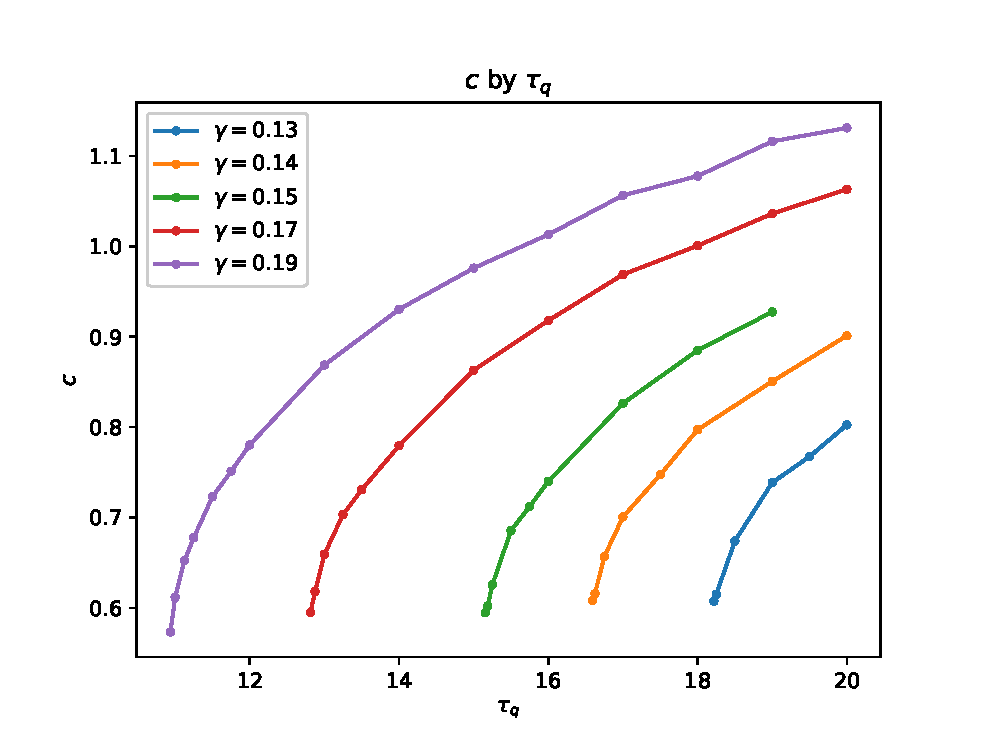
\includegraphics[width=.9\linewidth]{pulse_bifurcation}
%	\end{center}
%}

%%%%%%%%%%%%%%%%%%%%%%%%%%%%%%%%%%%%%%%%%%%%%%%%%%%%%%%%%%%%%%%%%%%%%%%%%%%%%%
\headerbox{Wave Response}{name=response,column=2}%,above=solutions2}
{
	\begin{itemize}
	\item These solutions have fixed speeds.
	\item Our visual system is capable of tracking and predicting the location of objects with a variety of speeds.
	\item \textbf{Can we augment the model in a biologically realisitc way to account for this variation in speed?}
	\item These waves are \textit{marginally stable} -- when stimulated, they tend toward a translate of the original traveling wave. Below we see snapshots for $\varepsilon I_u = 0.1 \delta(t - 20)$.
	\begin{center}
		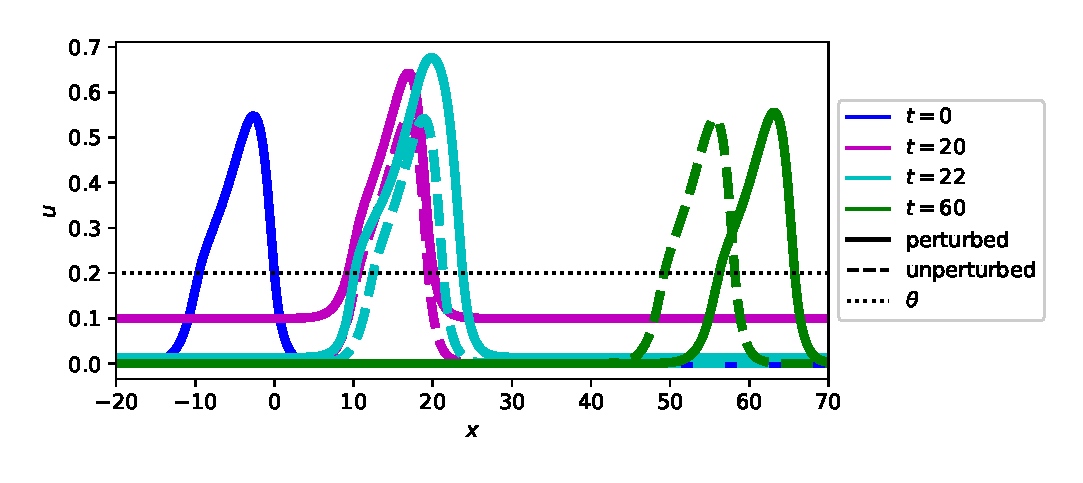
\includegraphics[width=.9\linewidth]{response_example}
	\end{center}
	\item The amount of translation is called the \textit{wave response}, denoted $\nu(t)$.
	\end{itemize}
	\vspace{.2cm}
}

%%%%%%%%%%%%%%%%%%%%%%%%%%%%%%%%%%%%%%%%%%%%%%%%%%%%%%%%%%%%%%%%%%%%%%%%%%%%%%
\headerbox{Asymptotics}{name=asymptotics,column=2,below=response,above=bottom}
{
	\begin{itemize}
		\item Expand about the traveling wave solution
		\begin{align*}
			u(\xi, t) &= U(\xi - \varepsilon \nu(t)) + \varepsilon \phi(\xi, t) + \OO(\varepsilon^2) \\
			q(\xi, t) &= Q(\xi - \varepsilon \nu(t)) + \varepsilon \psi(\xi, t) + \OO(\varepsilon^2)
		\end{align*}
		\item Substitute into the model, linearize, and extract the $\OO(\varepsilon)$ equation:
		\begin{align*}
   		\begin{bmatrix}\tau_u & 0 \\ 0 & \tau_q\end{bmatrix} \begin{bmatrix}\phi \\ \psi \end{bmatrix}_t + \LL \left(\begin{bmatrix} \phi \\ \psi \end{bmatrix} \right)
       = 
       \underbrace{\begin{bmatrix} I_u + \tau_u U' \nu' \\ I_q + \tau_q Q' \nu ' \end{bmatrix}}_{\text{RHS}}
		\end{align*}
		where
		\begin{align*}
		\LL \left(\begin{bmatrix} \phi \\ \psi \end{bmatrix} \right) = \begin{bmatrix}\phi \\ \psi \end{bmatrix} - c\begin{bmatrix}\tau_u & 0 \\ 0 & \tau_q\end{bmatrix} \begin{bmatrix}\phi \\ \psi \end{bmatrix}_\xi +
		\begin{bmatrix}
  -w Q f'(U) * \cdot  & -w f(U) * \cdot \\
  \beta Q f'(U) & \beta f(U)
		\end{bmatrix}
		\begin{bmatrix}\phi \\ \psi \end{bmatrix}
		\end{align*}
		\item We apply the \textbf{Fredholm alternative}: A unique bounded solution exists if the right-hand-side is orthogonal to the null-space of the adjoint.
		\item The one-dimensional null-space $(v_1, v_2) \in \mathcal{N}(\LL^*)$ satisfies
		\begin{align*}
	    	-c \tau_u v_1' &= v_1 -f'(U)Q \int_\RR w(|y-\xi|) v_1(y) \ dy + \beta Q f'(U)v_2 \\
	    	-c \tau_q v_2' &= v_2 - f(U) \int_\RR w(|y-\xi|) v_1(y) \ dy + \beta f(U) v_2.
		\end{align*}
		\item \textbf{Asymptotic approximation}:
		 \[
	 		\nu(t) = - \frac{\int_\RR v_1 \int_0^t I_u(\xi, \tau) \ d\tau + v_2 \int_0^t I_q(\xi, \tau) \ d\tau \ d\xi}{\int_\RR \tau_u U' v_1 + \tau_q Q' v_2 \ d\xi}.
	 	\]
	\end{itemize}
	
	\vspace{.2cm}
}

%%%%%%%%%%%%%%%%%%%%%%%%%%%%%%%%%%%%%%%%%%%%%%%%%%%%%%%%%%%%%%%%%%%%%%%%%%%%%%
\headerbox{Results}{name=results,column=3,row=0}
{
	\begin{itemize}
		\item Front null-space:
		\begin{align*}
			v_1(\xi) &= H(\xi) e^{-\xi/c\tau_u} \\
			v_2(\xi) &= \frac{c\tau_u}{2(1+c\tau_u)(1+\beta+c\tau_q)} \big( H(-\xi)e^{\xi} + H(\xi) e^{-\xi/c\tau_q} \big)
		\end{align*}
		\begin{center}
			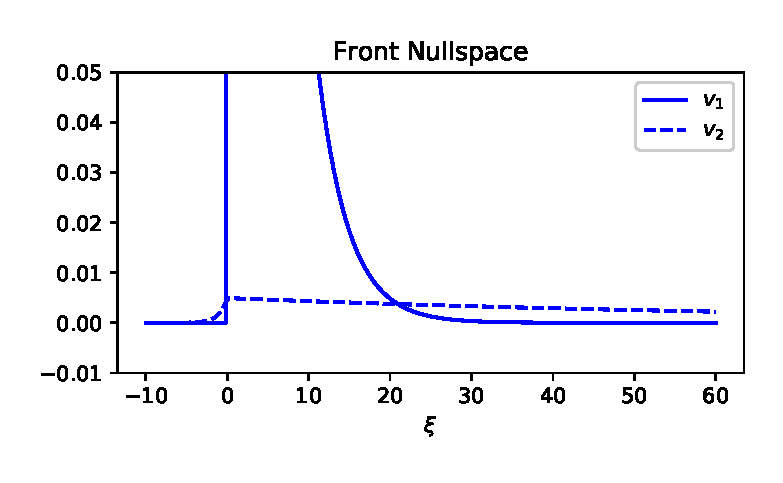
\includegraphics[width=.9\linewidth, trim={0cm, .2cm, 0cm, .2cm}, clip=true]{nullspace}
		\end{center}
		\vspace{-.5cm}
		\item Front response to global stimulus $\varepsilon I_u = \varepsilon \delta(t)$.
		\begin{center}
			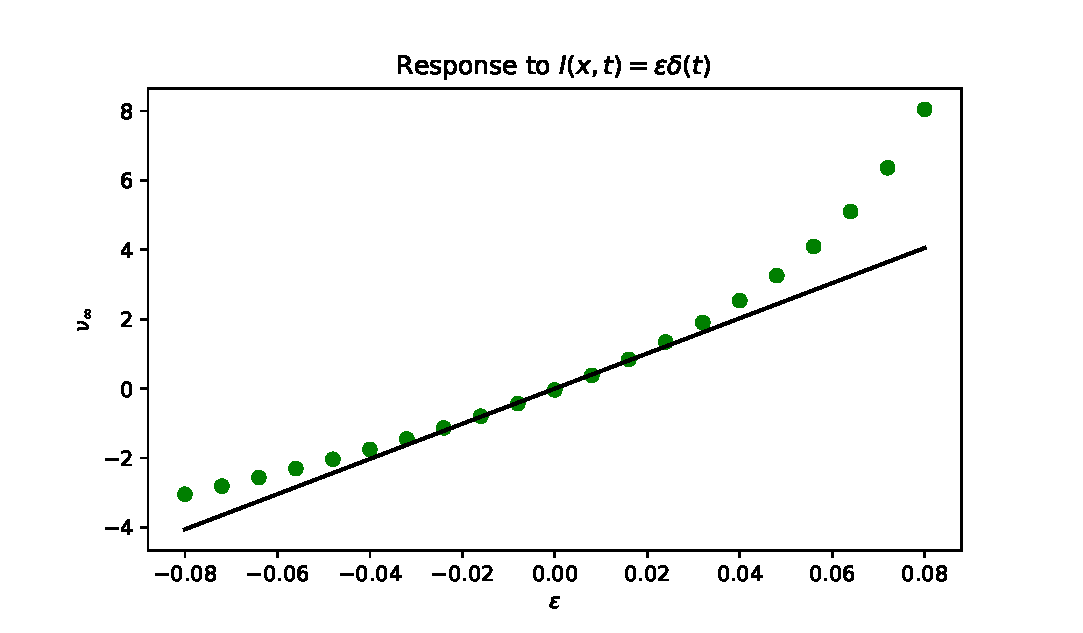
\includegraphics[width=.9\linewidth, trim={0cm, .2cm, 0cm, .2cm}, clip=true]{fig_spatially_homogeneous_limit}
		\end{center}
		\vspace{-.5cm}
		\item Pulse response to unit-width square pulse centered at $x_0$. 
		\[
			\varepsilon I_u = \tfrac{1}{20} \delta(t) I_{(x_0 - .5, x_0 + .5)}
		\]
		\begin{center}
			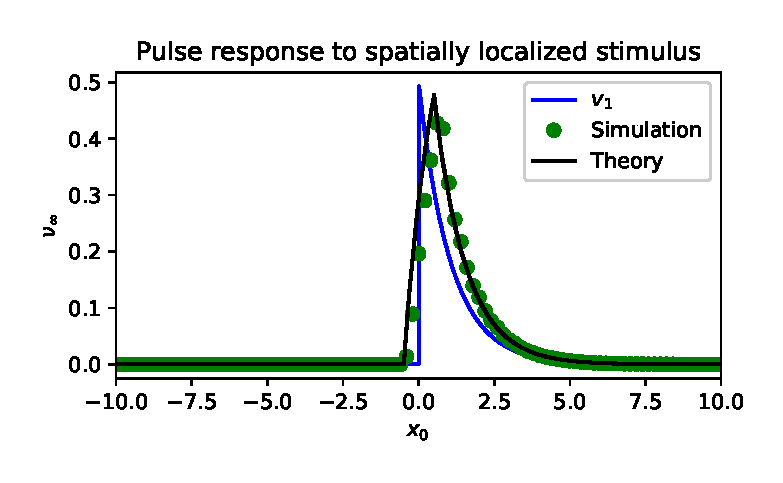
\includegraphics[width=.9\linewidth, trim={0cm, 0cm, 0cm, .2cm}, clip=true]{spatially_localized}
		\end{center}
	\end{itemize}
}

%%%%%%%%%%%%%%%%%%%%%%%%%%%%%%%%%%%%%%%%%%%%%%%%%%%%%%%%%%%%%%%%%%%%%%%%%%%%%%
\headerbox{References, Funding, and Links}{name=references,column=3,below=results,above=bottom}
{
\begin{minipage}{.7\textwidth} \begin{itemize}
		\item Tsodyks, et al. (1998) Neural Computation
		\item Kilpatrick \& Bressloff (2010) Physica D 
		\item Kilpatrick \& Ermentrout (2012) Phys. Rev. E
	\end{itemize}
This work was supported by NSF DMS-2207700.
\end{minipage}
\begin{minipage}{.25\textwidth}

\includegraphics[width=\linewidth, trim={.7cm, .7cm, .7cm, .7cm}, clip=true]{QR}
%\includegraphics[width=\linewidth, trim={.7cm, .7cm, .7cm, .7cm}, clip=true]{NSF_logo}
\end{minipage}
\bigbreak

\texttt{https://shawsa.github.io/presentations/20230310} \texttt{\_recruitment\_poster.html}
	
}

\end{poster}
\end{document}
